\documentclass[wmii, inf, inz]{uwmthesis}
\usepackage[polish]{babel} \usepackage[utf8]{inputenc}
\usepackage[T1]{fontenc}
\usepackage[utf8]{inputenc}
\usepackage[MeX]{polski}
\usepackage{url}
\usepackage{tikz}
\usepackage{pgfplots}
\usepackage{pgfplotstable}
\usepackage{lmodern}
\usepackage{cleveref}
\usepackage{geometry}
\usepackage{tabularx}
\usepackage{float}
\newgeometry{tmargin=2.5cm, bmargin=2.5cm, lmargin=3.5cm, rmargin=2cm}
\pgfplotsset{compat=1.16}
\widowpenalty10000  
\clubpenalty10000 
\linespread{1.1}
\date{2019}
\title{Symulacja ruchu drogowego na skrzyżowaniu z~sygnalizacją świetlną sterowaną algorytmem ewolucyjnym}
\author{Krzysztof Pietraszko}
\etitle{Traffic simulation on junction with traffic lights controlled by an evolutionary algorithm}
\wykonanaw{Katedrze Metod Matematycznych Informatyki}
\ewykonanaw{the Department of Mathematical Methods in Computer Science}

\podkierunkiem{Dr Inż. Bartosza Nowaka}
\epodkierunkiem{Dr Inż. Bartosz Nowak}

\begin{document}
	\pgfplotstableread[col sep = comma]{evolutionLog.csv}\loadedtable
	\maketitle
	\chapter*{Streszczenie}
	\chapter*{Abstract}
The goal of the thesis was to implement an evolutionary algorithm that optimises traffic lights on a junction. \\
Evolutionary algorithms are a category of artificial intelligence techniques. They are widely used to solve optimisation problems. Their main mechanisms are inspired by the evolution of species. \\
Traffic lights improvement was presented as an optimisation problem with a goal function dependant on a simulation of the traffic. Unity engine and C\texttt{\#} language were used to implement the application. It performs the optimisation process with settings provided by the user. This thesis describes the algorithm and the functionality of the application itself. The results of optimisation were presented in the form of charts. Possible directions for further extension of the application were also proposed.
	\tableofcontents
	\chapter*{Wstęp}
%Wstęp od stworzenia swiata: komputery są pomocne również w zadaniach inżynieryjnych takich jak problemy optymalizacyjne np problem ustawienia optymalnych czasów (jak to ująć?)
\paragraph{}Komputery są obecnie niezwykle popularnymi urządzeniami znajdującymi zastosowanie w wielu dziedzinach życia. Są pomocne także w zadaniach inżynieryjnych takich jak problemy optymalizacyjne.
\section*{Problemy optymalizacyjne}
Problemy w wielu obszarach matematyki, inżynierii, ekonomii, medycyny i statystyki mogą być przedstawione w kategoriach optymalizacji.\\
Określenie problemu optymalizacyjnego rozpoczyna się od ustalenia zbioru zmiennych niezależnych lub parametrów. Często formułuje się również ograniczenia, które wyznaczają dozwolone wartości zmiennych. Inną istotną składową problemu optymalizacyjnego jest funkcja celu, której wartość zależy od zmiennych. Rozwiązaniem takiego problemu jest zbiór dozwolonych wartości zmiennych, dla których funkcja przyjmuje optymalną wartość (minimalną lub maksymalną, zależnie od badanego zagadnienia)\cite{9780122839528}.
\paragraph{} Do rozwiązywania problemów optymalizacyjnych często stosowane są metody sztucznej inteligencji. Dostarczają lepszych, szybszych i bardziej precyzyjnych rozwiązań niż konwencjonalne techniki, szczególnie w złożonych problemach inżynieryjnych. Spośród ich charakterystycznych cech warto wymienić następujące:
\begin{itemize}
	\item Metody te ,,pamiętają'' swoje poprzednie odkrycia,
	\item Dostosowują swoją wydajność (np. decydują o eksploracji lub eksploatacji), co przekłada się na unikanie utknięcia w minimum lokalnym,
	\item Mogą planować swoje działania długofalowo~\cite{Badar2013StudyOA}.
\end{itemize}
\section*{Algorytmy ewolucyjne} Przykładowym typem metod sztucznej inteligencji są algorytmy ewolucyjne. Poszukują one optymalnego rozwiązania problemu w sposób, który czerpie inspirację z mechanizmu ewolucji gatunków. Jednym z głównych czynników wyróżniających ten zbiór technik jest to, że jednocześnie zmieniana jest pewna populacja rozwiązań, a jej przekształcenia przypominają procesy zachodzące w przyrodzie. Zrozumienie algorytmów ewolucyjnych wymaga przyswojenia pewnych kluczowych pojęć, takich jak dostosowanie (ang. \textit{fitness}) stanowiące ocenę danego rozwiązania, oraz krzyżowanie i mutacja będące mechanizmami przekształcania populacji. \\Krzyżowanie tworzy nowe rozwiązanie łącząc cechy dwóch innych, podczas gdy mutacja w losowy sposób modyfikuje istniejące rozwiązanie. 
Przebieg algorytmu genetycznego rozpoczyna się od utworzenia początkowej populacji rozwiązań, które zazwyczaj są generowane losowo. W związku z tym zakłada się, że jest to różnorodny zbiór zawierający dobre i złe cechy.
Algorytm następnie generuje szereg kolejnych populacji (pokoleń), z pomocą wyżej wspomnianych mechanizmów przekształcających~\cite{Cohoon:2003:EAP:903758.903786}. Kluczowe jest tu zachowanie równowagi między wykorzystywaniem znanych pozytywnych cech (a więc krzyżowaniem) a odkrywaniem nowych możliwości w przestrzeni dopuszczalnych rozwiązań (a więc mutacją). Istnieją modele mające na celu zmniejszenie tego problemu. Przykładowo działanie algorytmu można podzielić na fazy: pozyskiwania, akumulacji i wykorzystywania wiedzy~\cite{10.1371/journal.pone.0095693}. Innym rozwiązaniem jest przyjęcie zmiennego współczynnika mutacji danego pewną funkcją. Taką technikę przyjęto w tej pracy. 
\section*{Przykładowe zastosowania algorytmów ewolucyjnych} Do ciekawych zastosowań algorytmów ewolucyjnych należą m.in. antena statku kosmicznego~\cite{Lohn2006AutomatedAD}, czy też wentylator silnika~\cite{article}, których kształt został zaprojektowany przez taki algorytm. Obszary przejawiające duży potencjał to chociażby planowanie produkcji~\cite{Wall:1996:GAR:925320}, przewidywanie zmian temperatury na Ziemi\cite{Stanislawska:2012:MGT:2400749.2401077} i wiele innych~\cite{Steinbuch2010}.
\paragraph{}W tej pracy omówiono wykorzystanie algorytmu ewolucyjnego do usprawnienia płynności ruchu drogowego na skrzyżowaniu poprzez optymalizację sygnalizacji świetlnej. Stworzono aplikację przeprowadzającą proces uczenia z możliwością konfiguracji jego ustawień. Efektem końcowym pracy aplikacji jest wyświetlenie optymalnych parametrów sygnalizacji.
\section*{Usprawnienie sygnalizacji świetlnej jako problem optymalizacyjny}
Każda zmienna niezależna to czas, przez jaki wybrane sygnalizatory są zielone. Ewaluacja funkcji celu każdorazowo wymaga przeprowadzenia symulacji ruchu pojazdów, którą w tym celu zaimplementowano. Symulacja trwa dopóki określona liczba samochodów nie opuści skrzyżowania, a czas jej trwania decyduje o ocenie danego osobnika. \\
{\Huge TODO: OPIS ROZDZIAŁÓW}

	\chapter*{Użyte technologie}
Głównymi czynnikami decydującymi o doborze technologii były
\begin{itemize}
	\item Prostota interakcji z kartą graficzną,
	\item Dobre narzędzia do debugowania kodu,
	\item Jakość i kompletność dokumentacji,
	\item Wydajność,
	\item Możliwość prostej implementacji interfejsu graficznego,
	\item Wcześniejsze doświadczenie,
	\item Szybkość kompilacji -- istotna przy częstych zmianach w kodzie.
\end{itemize}
\section*{Unity}
Unity to wieloplatformowy silnik autorstwa firmy Unity Technologies, którego głównym zastosowaniem jest tworzenie gier dwuwymiarowych i trójwymiarowych oraz symulacji. W porównaniu do podobnych narzędzi wyróżnia się prostotą obsługi, dużym naciskiem na edytory wizualne i zintegrowanym środowiskiem, które nie wymaga skomplikowanej konfiguracji. Wspiera wiele API graficznych (DirectX, OpenGL, Metal i Vulkan)\cite{UnityManualGraphicsApiSupport} pod wspólnym interfejsem. Dzięki temu twórcy mogą w łatwy sposób tworzyć wersje swoich aplikacji na wiele platform bez uciążliwego dostosowywania swojego kodu. Podobne uproszczenia dostępne są również w zakresie obsługi urządzeń wejścia (jak mysz, klawiatura, kontrolery, ekrany dotykowe), a także dźwięku. Na wspomnienie zasługuje również wbudowany edytor WYSIWYG\footnote{WYSIWYG (What You See Is What You Get) - ,,otrzymujesz to co widzisz''} interfejsu graficznego aplikacji. Silnik można też rozszerzać o własne narzędzia, na przykład graficzny edytor krzywych. Programować swoją aplikację można jedynie w języku C\texttt{\#}~\cite{ProgramminginUnity}. Interfejs edytora Unity przedstawiono na rysunku~\ref{fig:unity}.
\section*{Język C\texttt{\#}}
C\texttt{\#} to silnie i statycznie typowany obiektowy język programowania zaprojektowany przez firmę Microsoft. Pozwala pisać kod z zachowaniem wszystkich założeń obiektowego paradygmatu programowania, czyli: abstrakcji, hermetyzacji, polimorfizmu i dziedziczenia. Mimo że C\texttt{\#} to język obiektowy, posiada wiele funkcji inspirowanych językami funkcyjnymi, które m.in. pozwalają bardzo łatwo dokonywać filtrowania, przekształcania czy sortowania kolekcji obiektów. Ułatwia to pisanie czytelnego, a przy tym zwięzłego, kodu. Pierwotnie kod C\texttt{\#} mógł być uruchamiany jedynie na systemie Windows. Zmieniło się to jednak w ostatnich latach dzięki środowiskom takim jak Mono oraz .NET Core i obecnie wspierane są inne platformy, takie jak Linux, macOS, iOS czy Android~\cite{Albahari2017}.
\begin{figure}[h!]
	\centering
	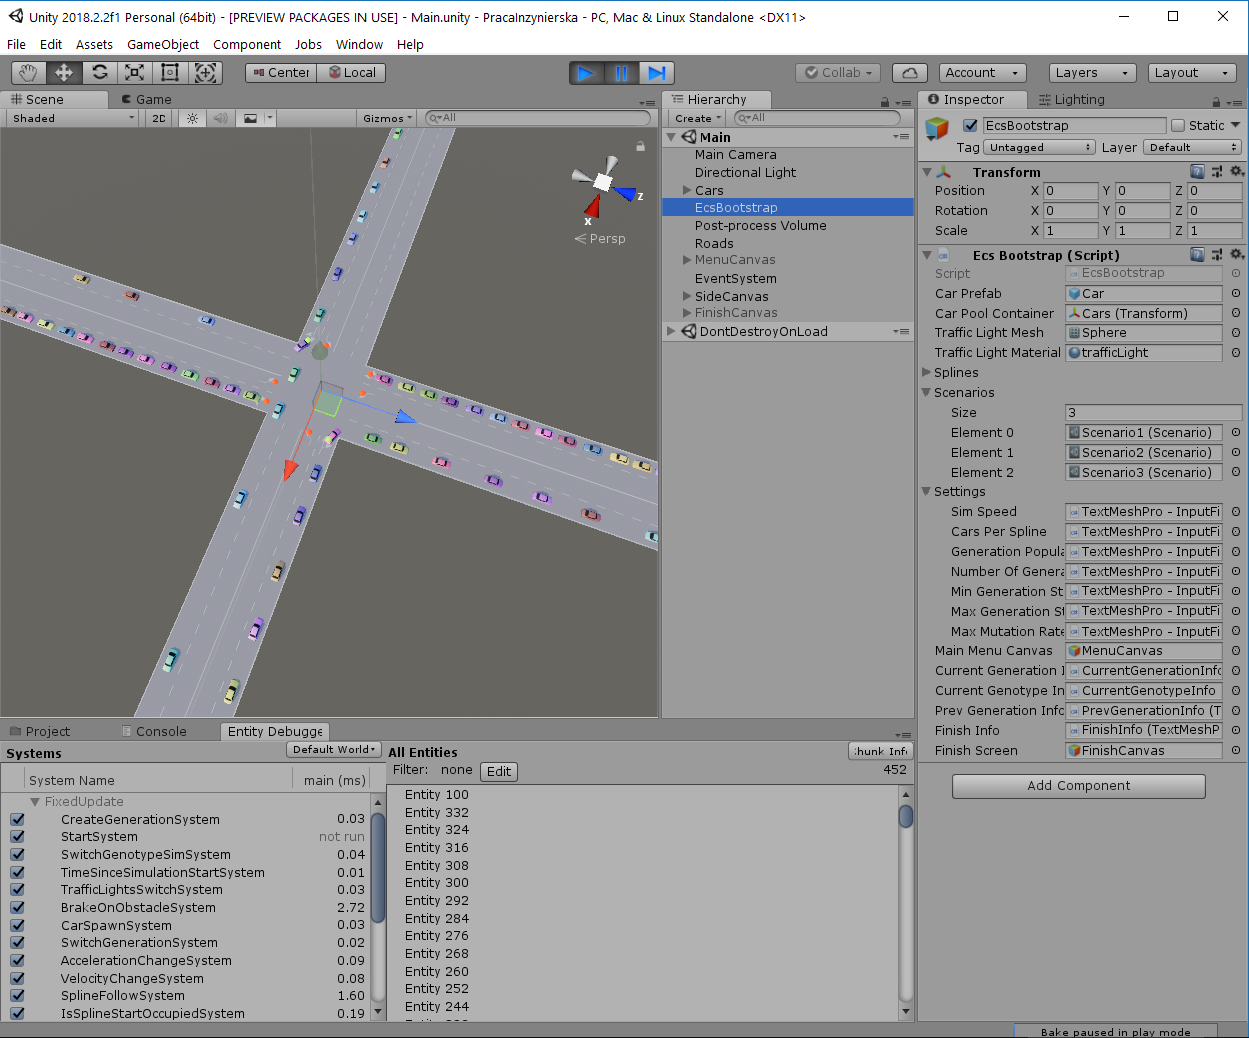
\includegraphics[width=1\linewidth]{unity}
	\caption[Interfejs edytora Unity]{Interfejs edytora Unity}
	\label{fig:unity}
\end{figure}
\section*{Inkscape}
Inkscape to darmowy program do tworzenia grafiki wektorowej. Tworząc w nim obrazy korzysta się z podstawowych kształtów takich jak elipsy, wielokąty, krzywe czy strzałki. Inkscape używa formatu Scalable Vector Graphics (SVG). Mimo że program opiera się na formacie wektorowym, plikiem wynikowym rysunku w tej pracy był obraz rastrowy, który można eksportować w dowolnej rozdzielczości. Decyzja ta wynika z ograniczeń w importowaniu grafik wektorowych w silniku Unity. Za użyciem Inkscape przemawiała przede wszystkim mnogość narzędzi i ustawień do tworzenia kształtów i wyrównywania ich położenia. Wygląd interfejsu programu przedstawiono na rysunku~\ref{fig:inkscape}. \\
W tej pracy został użyty do stworzenia grafiki skrzyżowania.
\begin{figure}
	\centering
	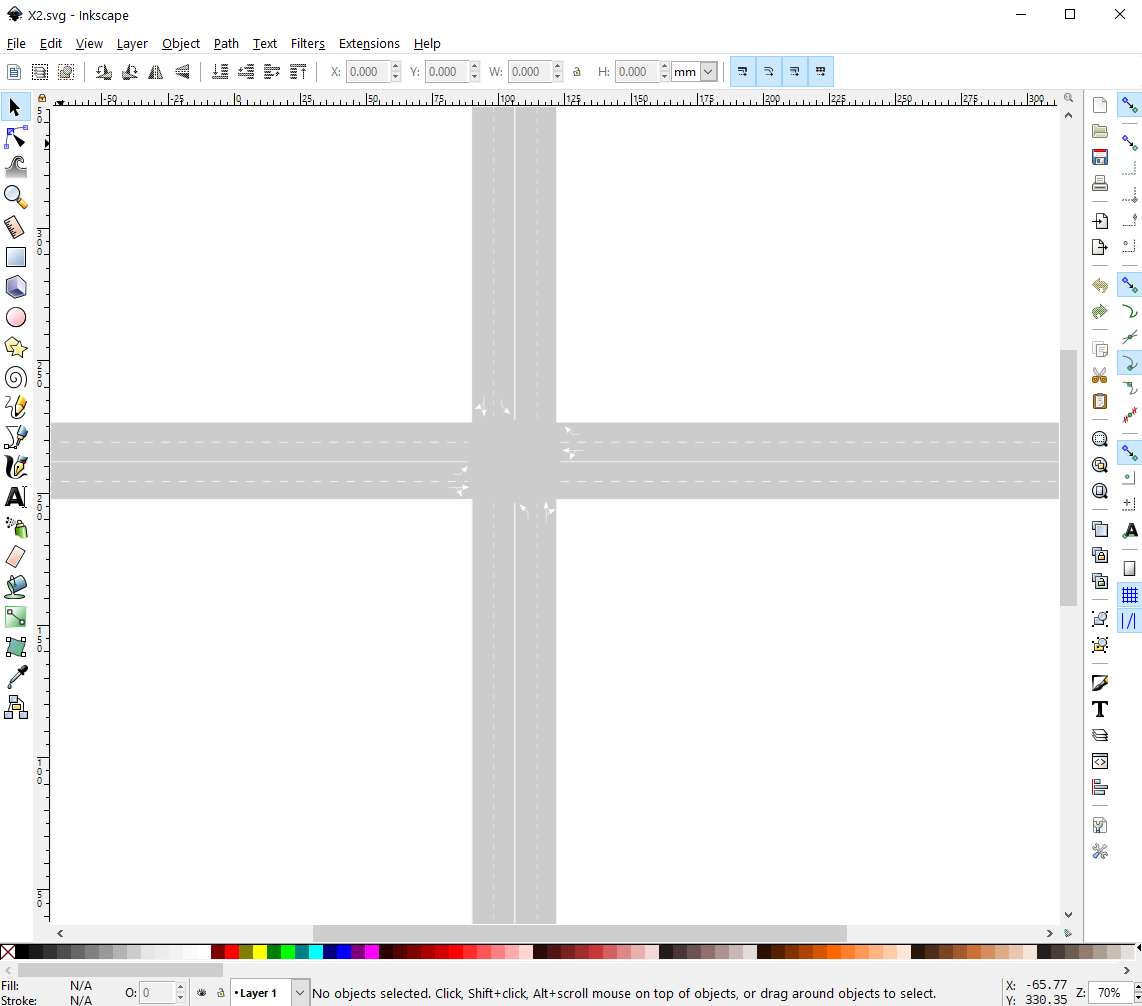
\includegraphics[width=1.0\linewidth]{inkscape}
	\caption[Interfejs programu Inkscape]{Interfejs programu Inkscape}
	\label{fig:inkscape}
\end{figure}
\section*{Blender}
Blender to darmowy program do tworzenia grafiki trójwymiarowej stworzony przez organizację Blender Foundation. Posiada narzędzia do modelowania, teksturowania, renderowania i animacji. Oprócz tego można z jego użyciem wykonywać proste symulacje fizyczne, a nawet zrealizować postprodukcję filmów. Niewątpliwie zaletą programu jest połączenie ogromnej liczby narzędzi w jeden pakiet. Dodatkowe atuty to dobra integracja z silnikiem Unity, wygoda użytkowania i wydajność. W tej pracy posłużył do wykonania trójwymiarowego modelu samochodu oraz ikony aplikacji. Interfejs Blendera przedstawia rysunek~\ref{fig:blender}.
\begin{figure}[h!]
	\centering
	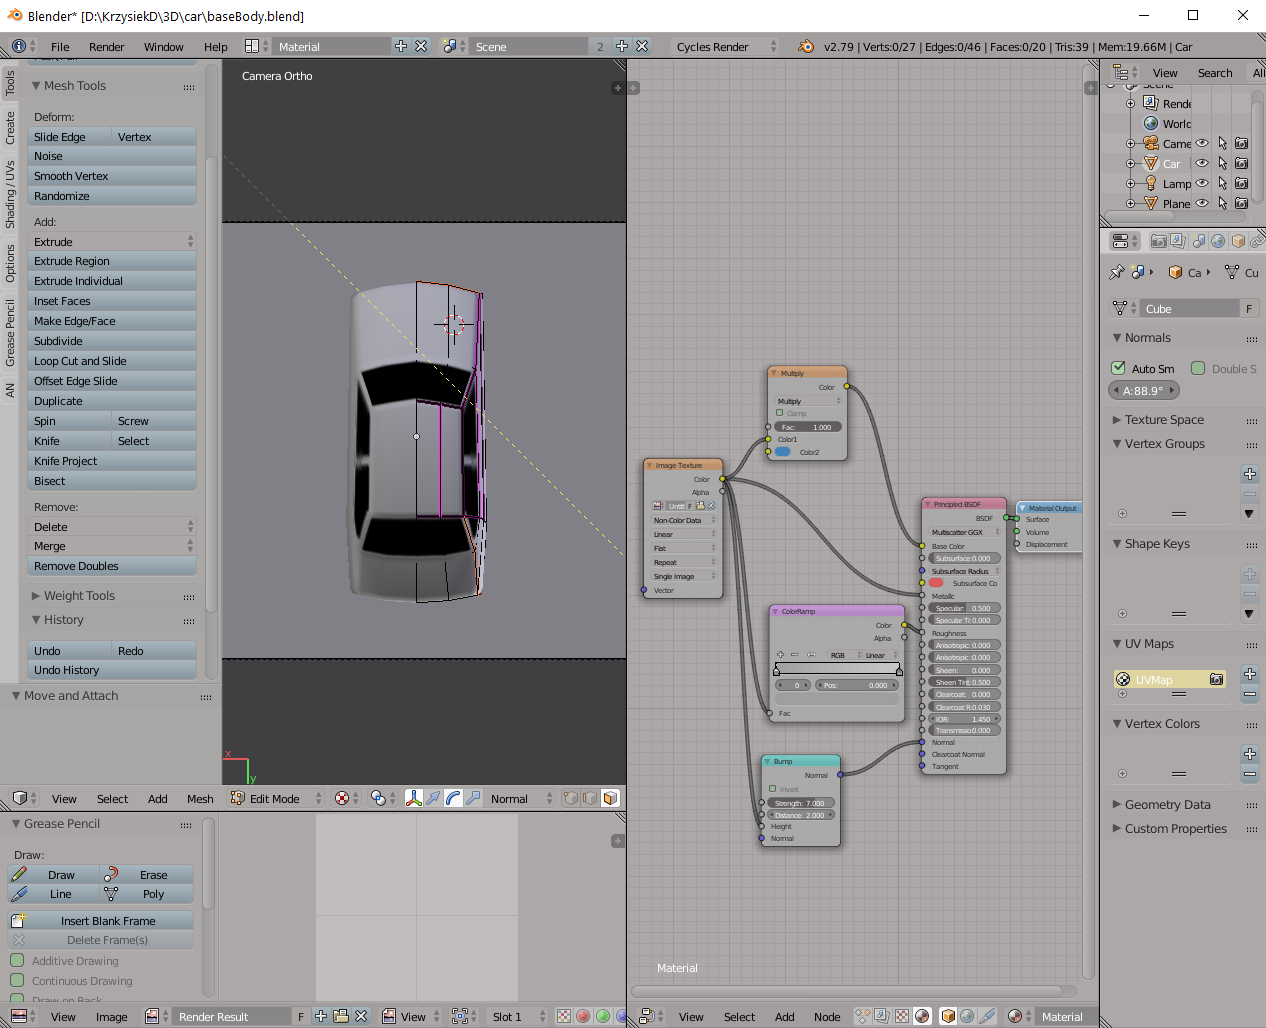
\includegraphics[width=1\linewidth]{blender}
	\caption[Interfejs programu Blender]{Interfejs programu Blender}
	\label{fig:blender}
\end{figure}


	\chapter*{Projekt aplikacji}
Aplikacja jest wysoce wyspecjalizowana -- przeprowadza wyłącznie proces symulacji i uczenia. Użytkownik może konfigurować ustawienia tego procesu.
\section*{Wymagania funkcjonalne}
\begin{itemize}
	\item Przeprowadzanie procesu uczenia optymalnych czasów świecenia sygnalizatorów na skrzyżowaniu za pośrednictwem algorytmu ewolucyjnego, wykorzystującego symulację ruchu pojazdów do oceny rozwiązań, 
	\item Konfiguracja ustawień symulacji, będącej bazą procesu uczenia,
	\item Konfiguracja ustawień algorytmu ewolucyjnego,
	\item Wyświetlanie na bieżąco informacji o przebiegu uczenia,
	\item Wyświetlenie wyników uczenia po jego zakończeniu.
\end{itemize}
\section*{Wymagania pozafunkcjonalne}
\begin{itemize}
	\item Stabilność -- aplikacja musi pracować bezawaryjnie przez wiele godzin,
	\item Wydajność -- aplikacja musi działać na tyle wydajnie, aby symulacja mogła być przeprowadzana kilkadziesiąt razy szybciej niż czas rzeczywisty.
\end{itemize}
\section*{Przypadki użycia}
W projekt występuje tylko jeden przypadek użycia: ,,Przeprowadź proces optymalizacji sygnalizacji świetlnej''. Przedstawia go diagram aktywności na rysunku~\ref{fig:diagramaktywnosci}. 
\section*{Przebieg przypadku użycia ,,Przeprowadź proces optymalizacji sygnalizacji świetlnej''}
Użytkownik najpierw może ustawić konfigurację symulacji oraz algorytmu ewolucyjnego. Następne wybiera scenariusz (czyli kolejność zapalania sygnalizatorów) co powoduje rozpoczęcie procesu uczenia. Aplikacja kolejno generuje, symuluje, a potem ocenia osobników pokolenia, jednocześnie wyświetlając na ekranie informacje o przebiegu uczenia. Pokolenia są kolejno generowane tak długo, aż zostanie osiągnięta ich liczba określona w konfiguracji. Następnie aplikacja wyświetla ekran końcowy prezentujący wyniki uczenia.
\begin{figure}[H]
	\centering
	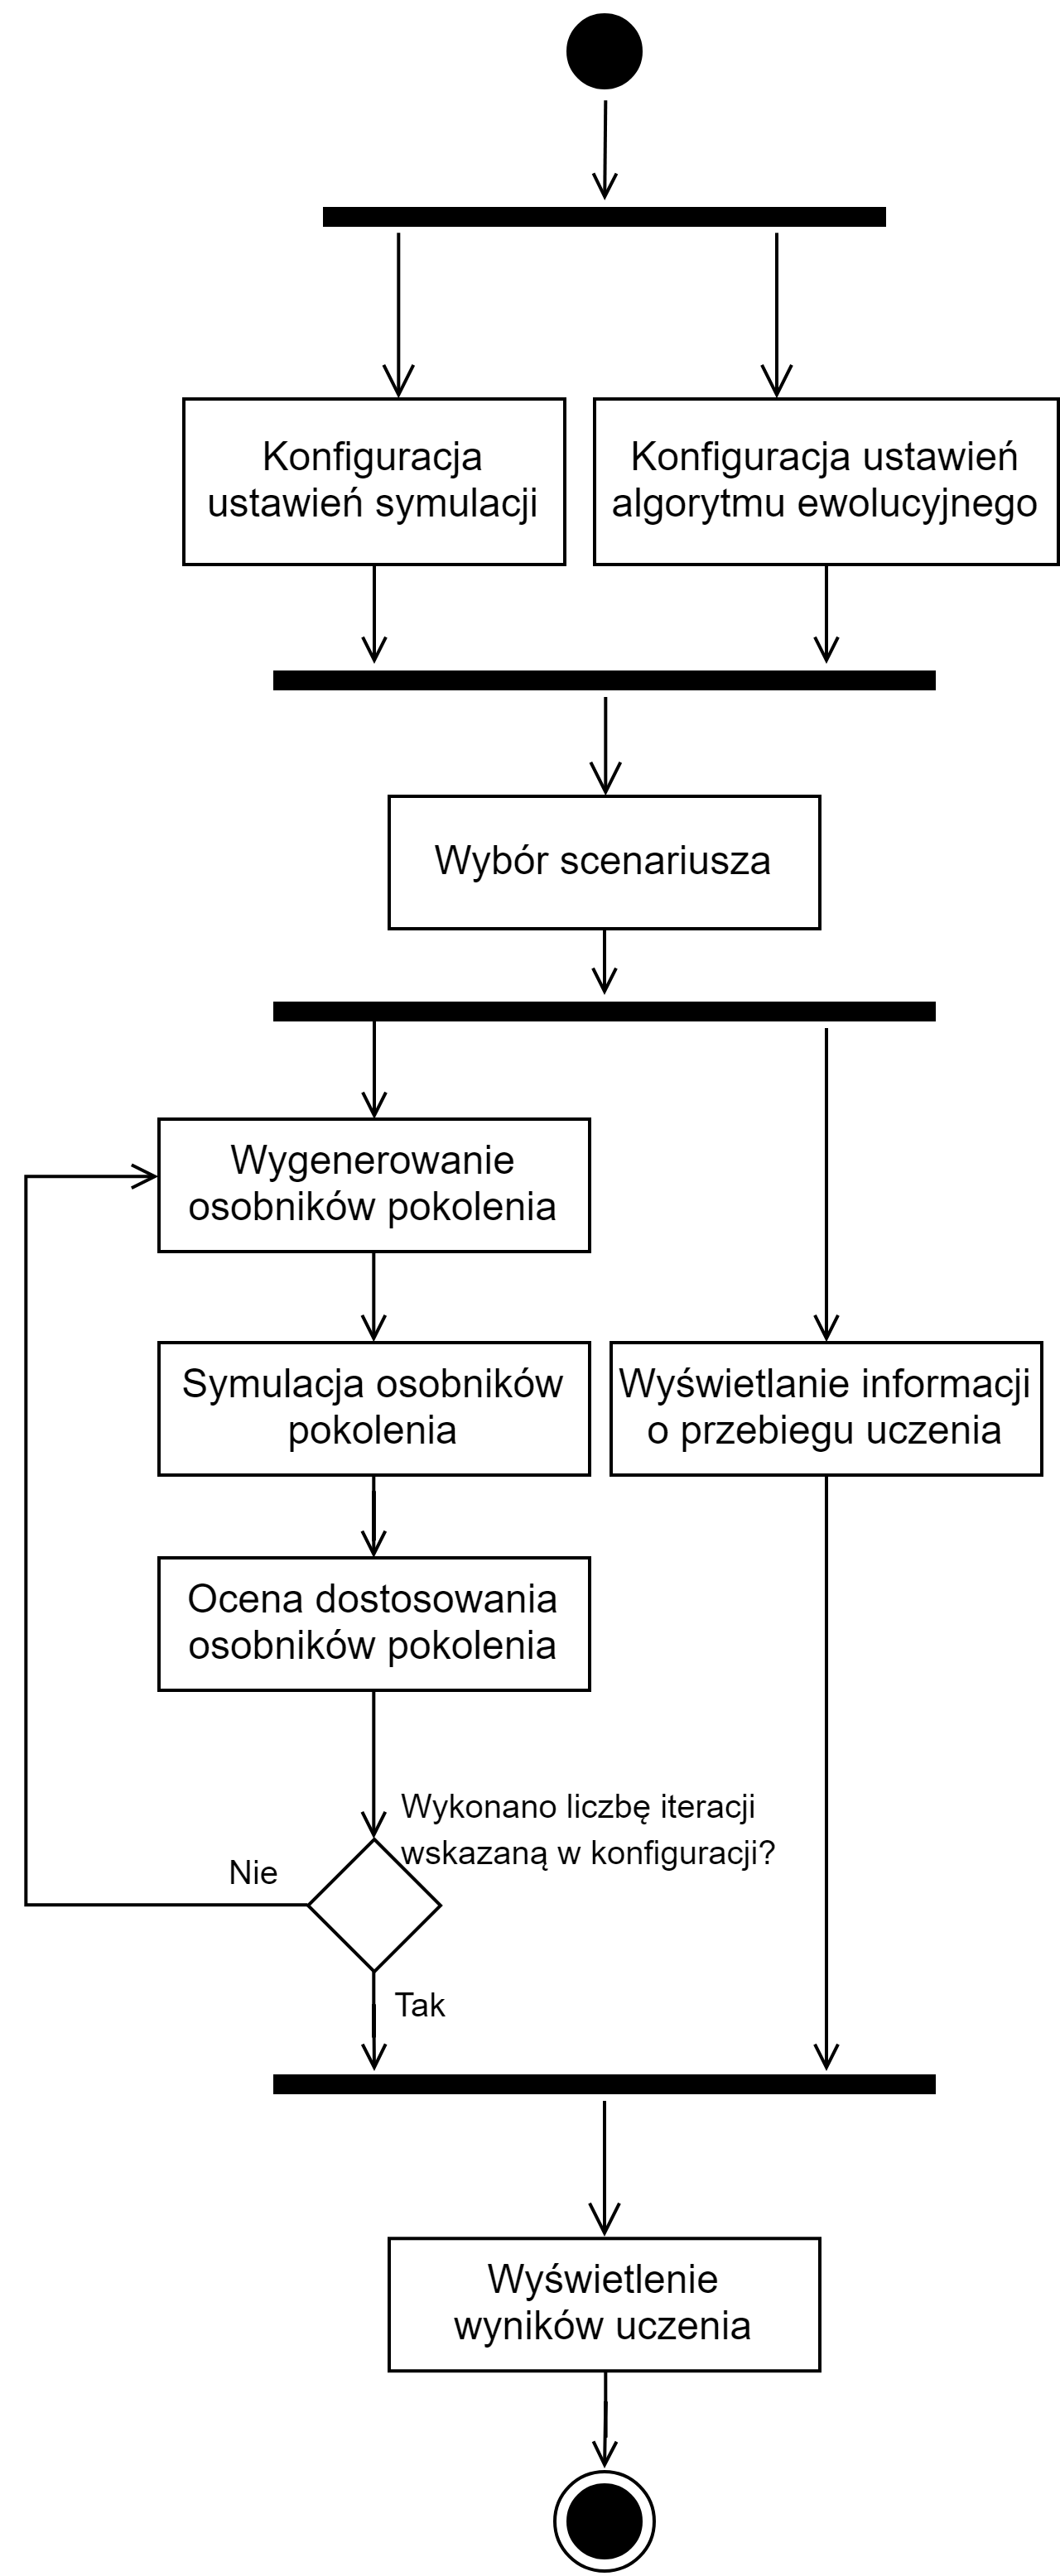
\includegraphics[height=0.8\textheight]{diagram_aktywnosci}
	\caption[Diagram aktywności przypadku użycia ,,Przeprowadź proces uczenia sygnalizacji'']{Diagram aktywności przypadku użycia ,,Przeprowadź proces uczenia sygnalizacji''}
	\label{fig:diagramaktywnosci}
\end{figure}

	\chapter*{Opis teoretyczny algorytmu ewolucyjnego}
Proces uczenia sygnalizacji świetlnej w tej pracy został zrealizowany z pomocą algorytmu ewolucyjnego. Ten rozdział opisuje kolejne kroki, z których składa się proces uczenia. Szczegóły dotyczące zastosowania poniższego algorytmu zostały opisane w następnym rozdziale.
\section*{Pierwsze pokolenie}
Przebieg uczenia rozpoczyna się od wygenerowania pierwszego pokolenia osobników. Osobnik to właściwie zbiór wartości określonych parametrów. W pierwszym pokoleniu wartości te generowane są losowo z zakresu określonego w konfiguracji algorytmu. 
\section*{Funkcja dostosowania}
Osobniki wygenerowanego pokolenia poddawane są ocenie, która określa ich dostosowanie (ang. \textit{fitness}). Funkcja dostosowania określona jest wzorem:
\begin{equation}
f(x) = max(t(1),\ldots, t(n)) - t(x)
\label{fitness}
\end{equation} 
gdzie:\\
\begin{tabularx}{\textwidth}{ r c l }
$x$ & -- & oceniany osobnik\\
$n$ & -- & liczba osobników w pokoleniu\\
$t(a)$ & -- & czas, w jakim określona liczba samochodów przejechała przez skrzyżowanie,\\ &&przy sygnalizacji ustawionej wg parametrów osobnika $ a $
\end{tabularx}
\section*{Generowanie nowego pokolenia}
Najlepszy osobnik poprzedniego pokolenia jest kopiowany wprost do nowego. 
Wybór reszty osobników odbywa się drogą selekcji turniejowej. Z poprzedniego pokolenia losowane są 3 osobniki. Spośród tych trzech wybierany jest ten o najwyższej wartości funkcji dostosowania. Taki turniej powtarzany jest $2n$ razy, gdzie $n$ to liczba osobników w pokoleniu (określona w konfiguracji algorytmu). Następnie ze zbioru $2n$ osobników wybieranych jest $n$ o najlepszej wartości funkcji dostosowania. Ta pula poddana jest następnie krzyżowaniu lub mutacji.
\section*{Mutacja i krzyżowanie}
Każdy osobnik z wygenerowanej puli, z wyjątkiem najlepszego zachowanego z poprzedniego pokolenia, zostaje zmutowany albo skrzyżowany z innym osobnikiem. Decyduje o tym ważone losowanie. Prawdopodobieństwo, że osobnik zostanie poddany mutacji jest zmienne i wyznacza je funkcja:
\begin{equation}
f(x) = (sin(x * \frac{1}{\frac{g}{1000}+\frac{x}{100}})+1) : 2 \cdot m
\label{mutRate}
\end{equation}
gdzie:\\
\begin{tabularx}{\textwidth}{ r c l }
	$x$ & -- & numer obecnego pokolenia\\
	$g$ & -- & liczba wszystkich pokoleń, określona w konfiguracji algorytmu\\
	$m$ & -- & maksymalny współczynnik mutacji, określony w konfiguracji algorytmu\\
	&&\\
\end{tabularx}\\
Wykres tej funkcji przedstawiono na rysunku~\ref{fig:mutRate}.\\
Korzyści wynikające ze stosowania dynamicznego współczynnika mutacji opisał Thierens~\cite{EvolutionaryComputation2002}. Również przy powstawaniu tej pracy zmienne prawdopodobieństwo mutacji okazało się lepszym rozwiązaniem w porównaniu do stałego współczynnika.

\begin{figure}[h]	
	\begin{tikzpicture}
	\begin{axis}
	[
	domain=0:110,
	width=\textwidth,
	xlabel=Pokolenie,
	ylabel=Współczynnik mutacji,
	xmin=0,
	xmax=110,
	ymin=0,
	ymax=1.05,
	samples=2000,
	xtick=100,
	xticklabel={$g$},
	ytick={\empty},
	extra y ticks={0,1},
	extra y tick labels={0,$m$},
	smooth
	]
	\addplot+[mark=none, black]{(sin(x * (1 / (0.1 + (x / 100.0)))*(180/3.14)) + 1.0)/2.0};
	\end{axis}
	\end{tikzpicture}
	\caption{Funkcja określająca współczynnik mutacji}
	\label{fig:mutRate}
\end{figure}
\pagebreak
Mutacja polega na losowym dodaniu lub odjęciu od wartości każdego parametru osobnika losowej liczby z zakresu 1--20. \\
Jeśli w wyniku wyżej opisanego losowania zostanie podjęta decyzja, że osobnik ma zostać poddany krzyżowaniu, to z puli losowo wybierany jest inny osobnik, od którego ten pierwszy przejmie wartość co drugiego parametru. Pozostałe parametry pozostają bez zmian.

Po zastosowaniu krzyżowania lub mutacji nowe pokolenie jest gotowe do oceny funkcją dostosowania opisaną wcześniej, co zamyka cykl. Kolejne pokolenia są generowane na postawie poprzednich i oceniane tak długo, aż osiągnięta zostanie liczba pokoleń określona w konfiguracji algorytmu.
	\chapter*{Opis aplikacji}
Po uruchomieniu aplikacji, użytkownikowi najpierw ukazuje się ekran ładowania (przedstawiony na rysunku~\ref{fig:splash}), a następnie menu główne (widoczne na rysunku~\ref{fig:ap1}).
\begin{figure}[h]
	\centering
	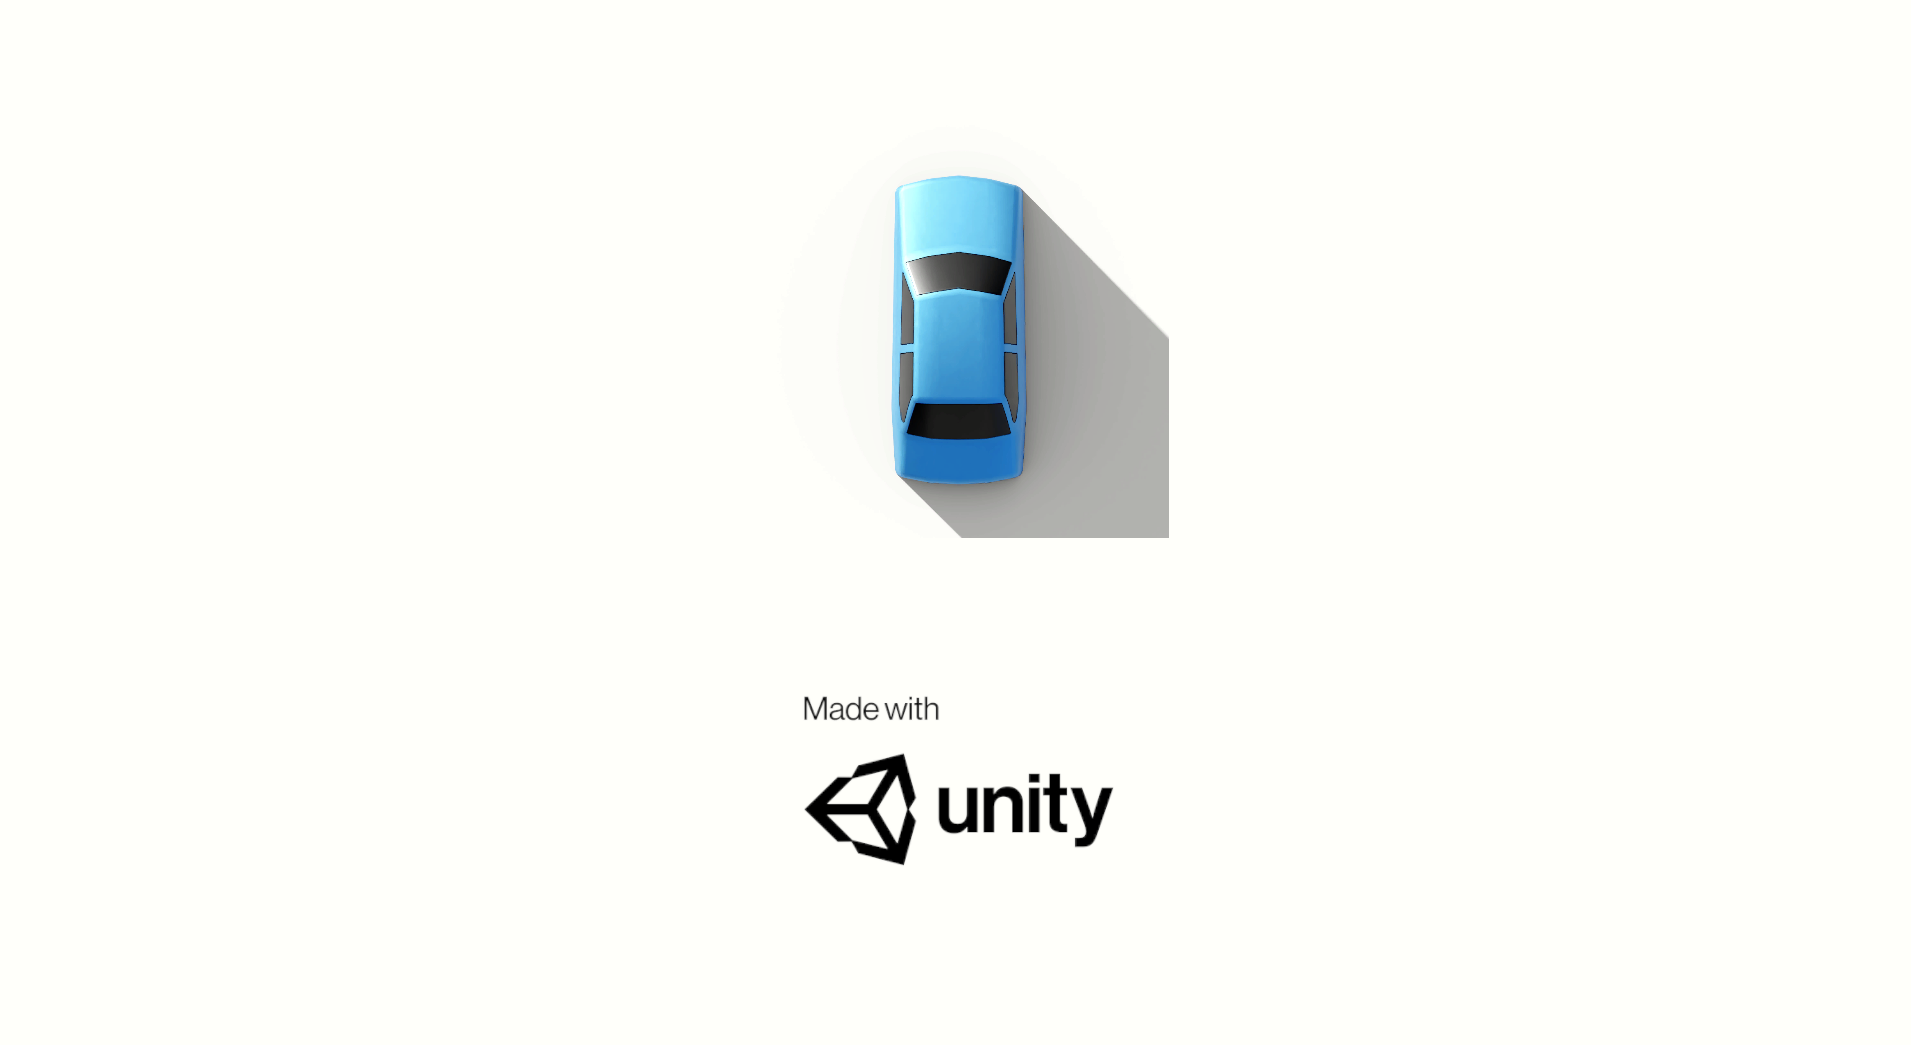
\includegraphics[width=1\linewidth]{splash}
	\caption[Ekran ładowania aplikacji]{Ekran ładowania aplikacji}
	\label{fig:splash}
\end{figure}

\section*{Menu główne}
W górnej części menu znajdują się pola liczbowe, do których użytkownik może wpisać ustawienia symulacji oraz algorytmu ewolucyjnego. Może też skorzystać z ustawień domyślnych. \\Dostępne ustawienia symulacji to:
\begin{itemize}
	\item Prędkość symulacji -- jest to mnożnik prędkości symulowania ruchu drogowego. Przy ustawieniu 1x przeliczane jest 30 kroków symulacji na sekundę. Jedynym górnym ograniczeniem tego ustawienia jest moc obliczeniowa procesora. Domyślna wartość to 100x. \\
	\item Liczba samochodów na pasie -- jest to liczba samochodów, które wjadą na każdy pas ruchu (pasy są widoczne w lewym dolnym rogu rysunku~\ref{fig:ap1}). Domyślna wartość to 20.\\
\end{itemize}
Ustawienia algorytmu ewolucyjnego przedstawiają się następująco:
\begin{itemize}
	\item Populacja pokolenia -- liczba osobników w każdym pokoleniu (stała $n$ w funkcji~\ref{fitness} w poprzednim rozdziale).\\
	\item Liczba pokoleń -- liczba pokoleń, po których proces uczenia ma zostać przerwany. Oprócz tego wpływa na współczynnik mutacji (stała $g$ w funkcji~\ref{mutRate} w poprzednim rozdziale).\\
	\item Długość kroku scenariusza -- zakres, w jakim muszą mieścić się wartości parametrów osobników, a więc długości kroków scenariusza.\\
	\item Maksymalny współczynnik mutacji -- stała $m$ w funkcji~\ref{mutRate} w poprzednim rozdziale.\\
\end{itemize}
\begin{figure}[h]
	\centering
	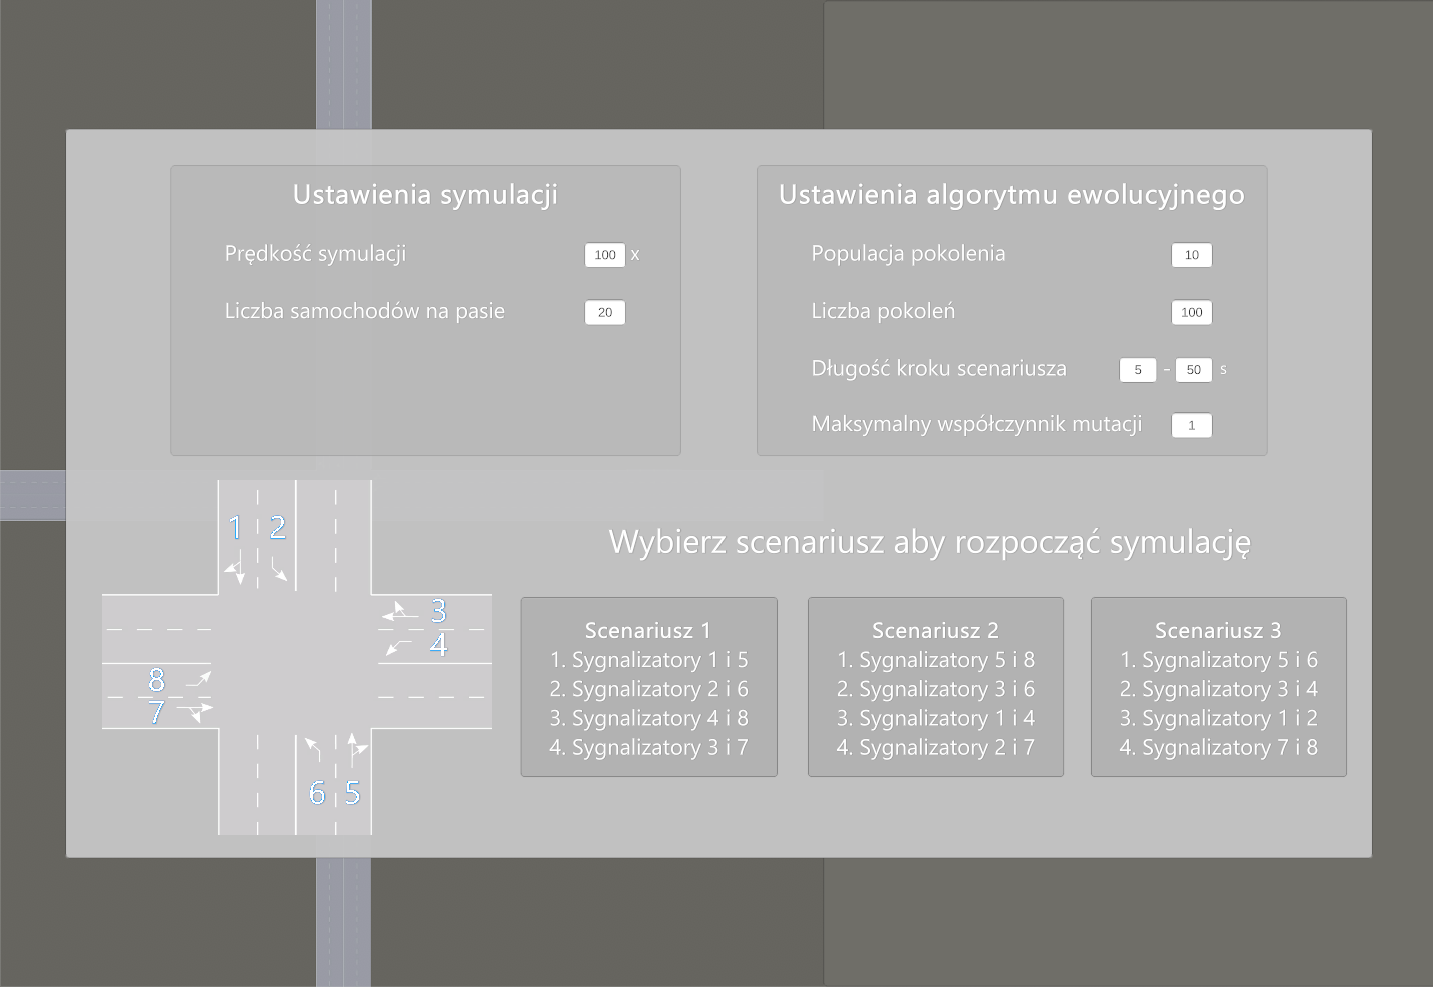
\includegraphics[width=1\linewidth]{ap1}
	\caption[Menu główne aplikacji]{Menu główne aplikacji}
	\label{fig:ap1}
\end{figure}
Po wybraniu ustawień użytkownik musi wybrać scenariusz. Jest to sekwencja sygnalizatorów, które będą zielone w określonym kroku scenariusza. W lewym dolnym rogu menu (na rysunku~\ref{fig:ap1}) widoczny jest schemat z ponumerowanymi sygnalizatorami, mający na celu ułatwienie użytkownikowi zrozumienia różnicy między scenariuszami. 
\section*{Scenariusz} Na przykładzie Scenariusza~1 widocznego w menu: podczas pierwszego kroku scenariusza zielone będą sygnalizatory nr 1 i 5 (oznaczone na schemacie po lewej), pozostałe zaś będą czerwone. Po przejściu do drugiego kroku zielone będą sygnalizatory nr 2 i 6, podczas gdy pozostałe będą czerwone. Analogicznie w kolejnych krokach scenariusza. Długość każdego z tych kroków opisuje obecnie symulowany osobnik.
\section*{Przebieg uczenia i symulacji ruchu}
Po wybraniu scenariusza rozpoczyna się proces uczenia. Aplikację podczas tego procesu przedstawia rysunek~\ref{fig:ap2}. Lewa część ekranu prezentuje postęp symulacji ruchu drogowego z zastosowaniem parametrów obecnie symulowanego osobnika. Z początkiem symulacji osobnika samochody wjeżdżają na skrzyżowanie i poruszają się zgodnie z sygnalizacją. Sygnalizatory przełączają się w odpowiednim czasie, a kiedy skończy się ostatni krok scenariusza, cykl sygnalizacji się zapętla -- wraca do pierwszego kroku. Symulacja trwa tak długo, aż wszystkie samochody opuszczą skrzyżowanie. Wtedy czas trwania symulacji jest zapisywany, zostanie później użyty do oceny dostosowania. Aplikacja przechodzi do symulacji kolejnego osobnika pokolenia -- na skrzyżowanie wjeżdża ta sama liczba samochodów, sygnalizacja zmienia się tym razem w odstępach określonych kolejnym osobnikiem. Cykl powtarza się, aż symulacji poddane zostaną wszystkie osobniki pokolenia. Następnie aplikacja dokonuje oceny i generuje nowe pokolenie, co opisano w rozdziale \textit{Opis teoretyczny algorytmu ewolucyjnego}. Potem odbywa się symulacja osobników nowego pokolenia. Cykl ten powtarza się, aż osiągnięta zostanie liczba pokoleń określona w konfiguracji. \\
Prawa część ekranu przedstawia stan uczenia -- numer obecnego pokolenia i osobnika. Po pierwszym pokoleniu dodatkowo w tej części wyświetlana jest informacja o tym, jaki był czas trwania symulacji najlepszego osobnika poprzedniego pokolenia. Prezentuje to rysunek~\ref{fig:ap3}. Z upływem pokoleń czas symulacji najlepszego osobnika spada, co jest widoczne, jeśli porówna się rysunek~\ref{fig:ap4} do rysunku~\ref{fig:ap3}.
\begin{figure}[h]
	\centering
	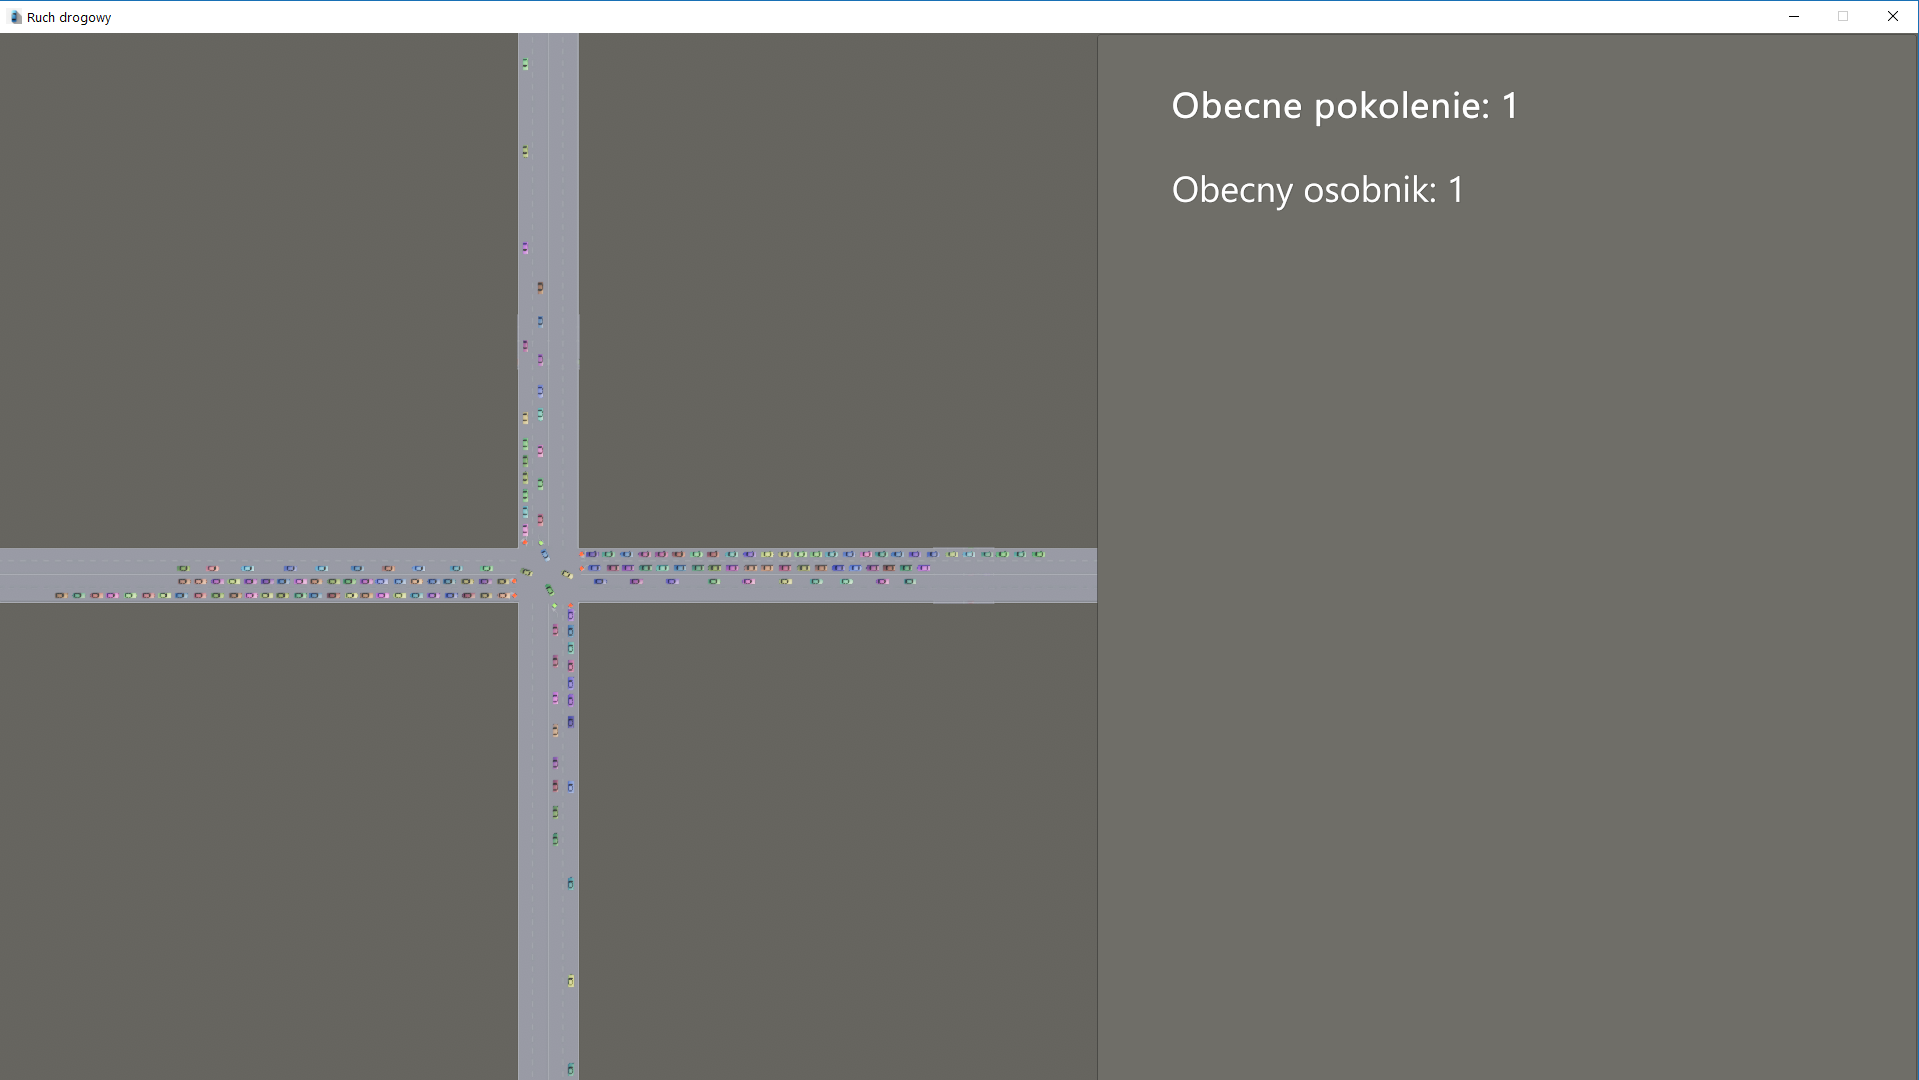
\includegraphics[width=1\linewidth]{ap2}
	\caption[Proces uczenia i symulacji ruchu]{Proces uczenia i symulacji ruchu podczas pierwszego pokolenia}
	\label{fig:ap2}
\end{figure}
\begin{figure}
	\centering
	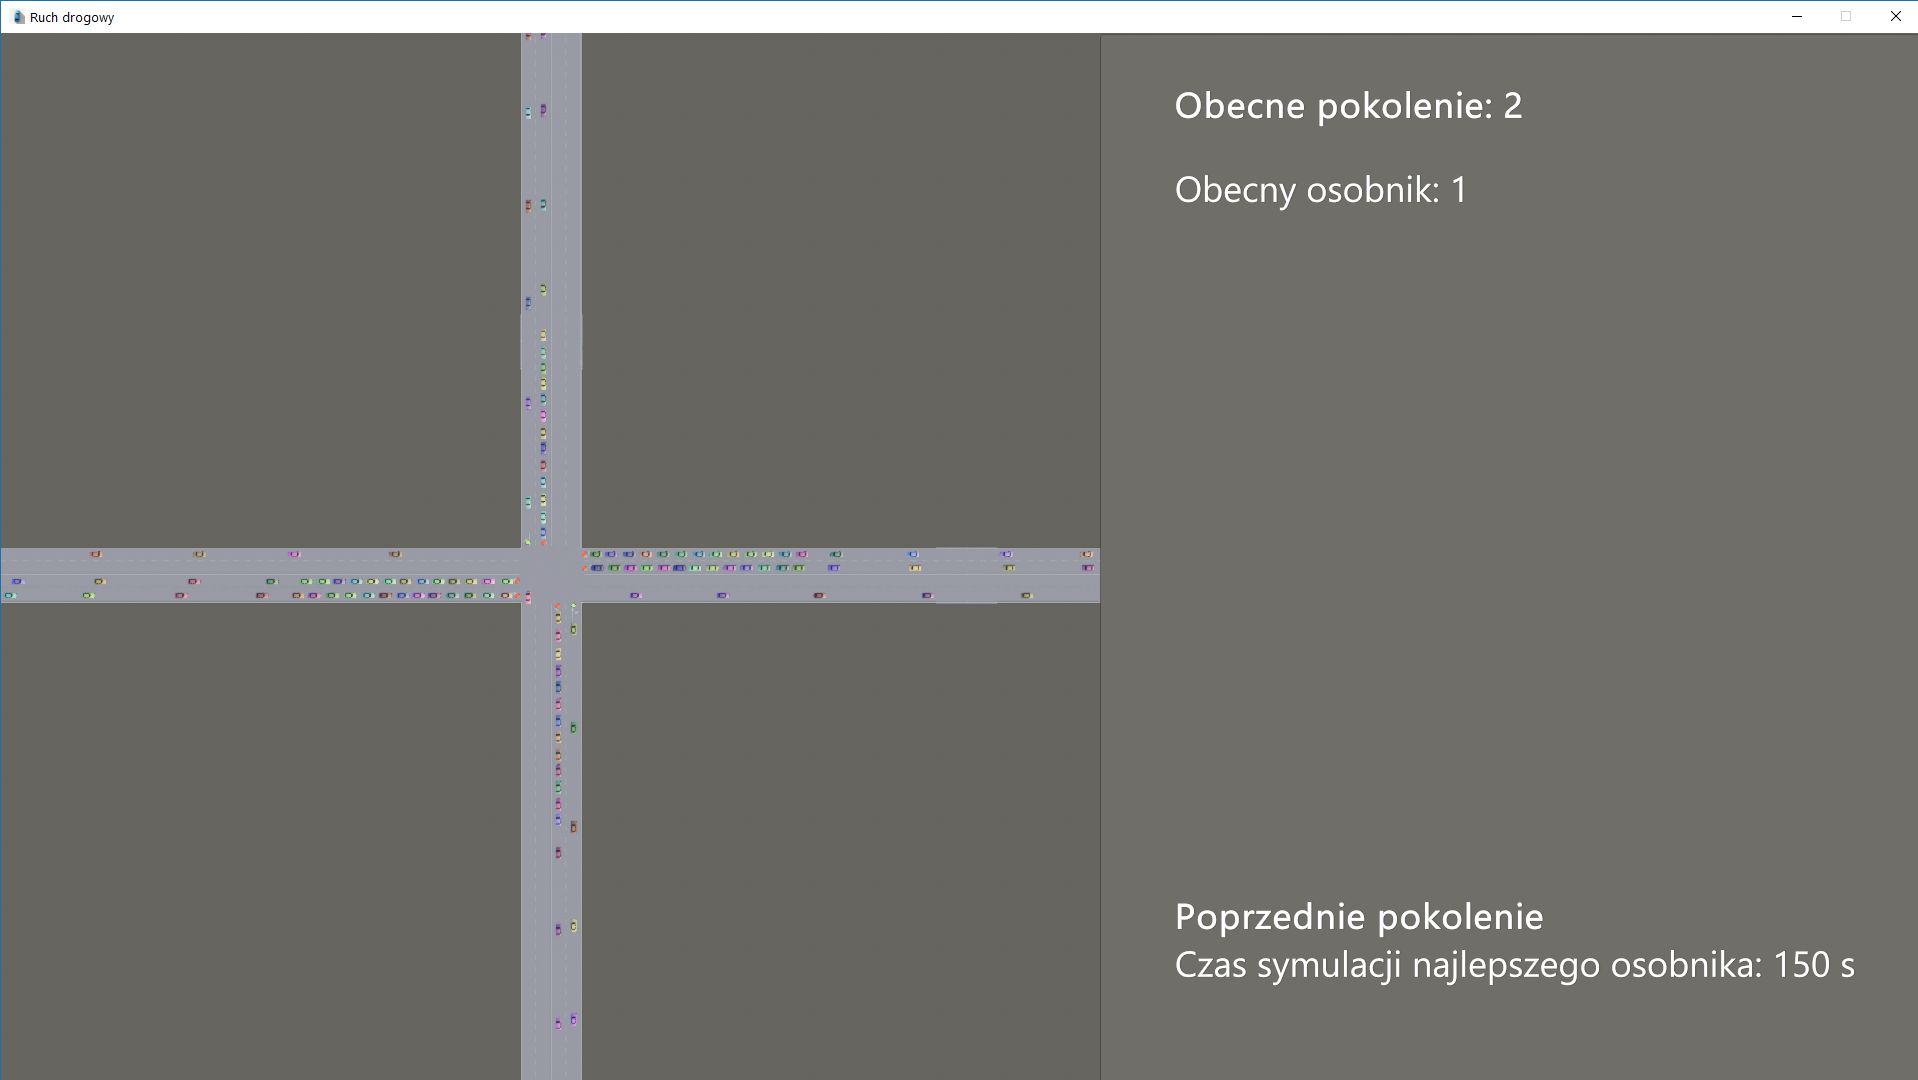
\includegraphics[width=1\linewidth]{ap3}
	\caption[Proces uczenia i symulacji ruchu]{Proces uczenia i symulacji ruchu podczas drugiego pokolenia}
	\label{fig:ap3}
\end{figure}
\begin{figure}
	\centering
	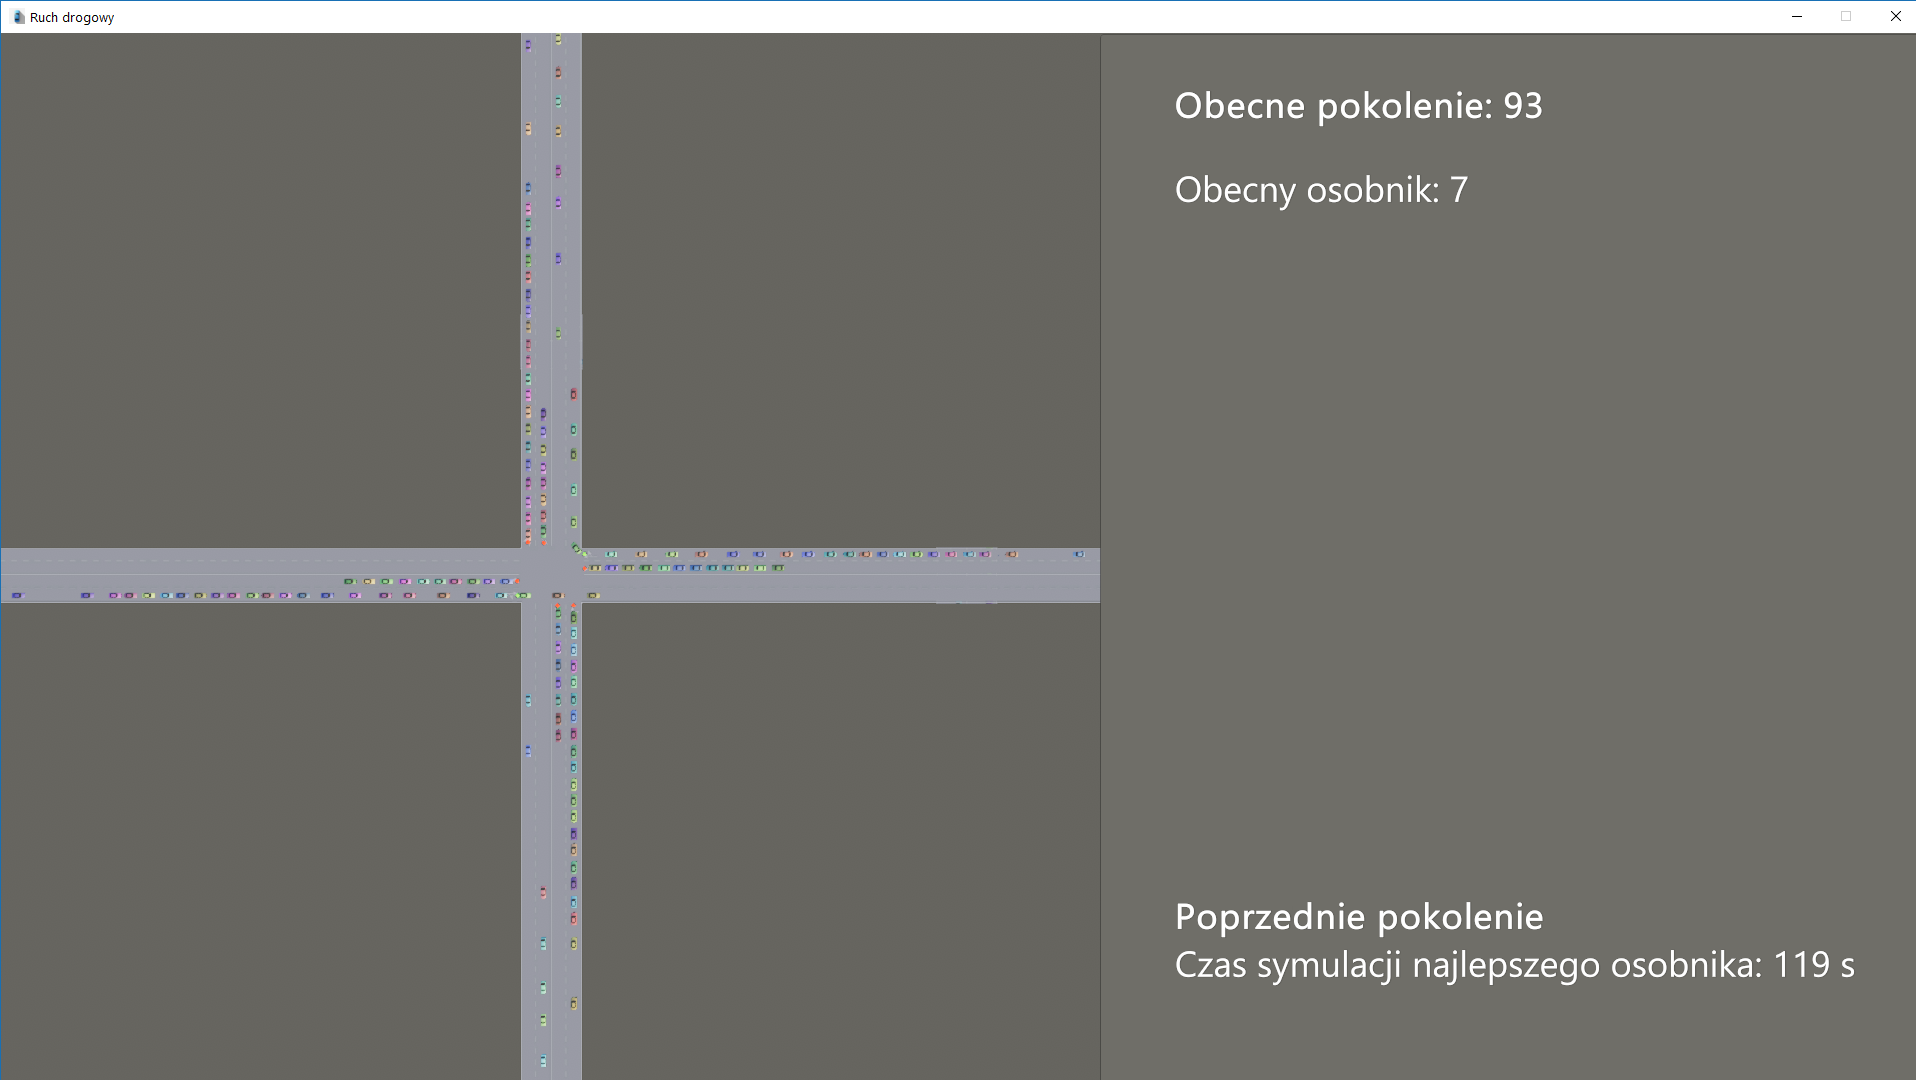
\includegraphics[width=1\linewidth]{ap4}
	\caption[Proces uczenia i symulacji ruchu]{Proces uczenia i symulacji ruchu podczas 93. pokolenia}
	\label{fig:ap4}
\end{figure}
\section*{Ekran końcowy}
Po ukończeniu procesu uczenia użytkownikowi ukazuje się ekran końcowy (widoczny na rysunku~\ref{fig:ap9}), który przedstawia wyniki uczenia. Informacje prezentowane na tym ekranie to czas trwania symulacji najlepszego osobnika ostatniego pokolenia i jego parametry. Na tym ekranie znajduje się również przycisk \textit{Wyjdź}, który pozwala na zamknięcie aplikacji.
\begin{figure}
	\centering
	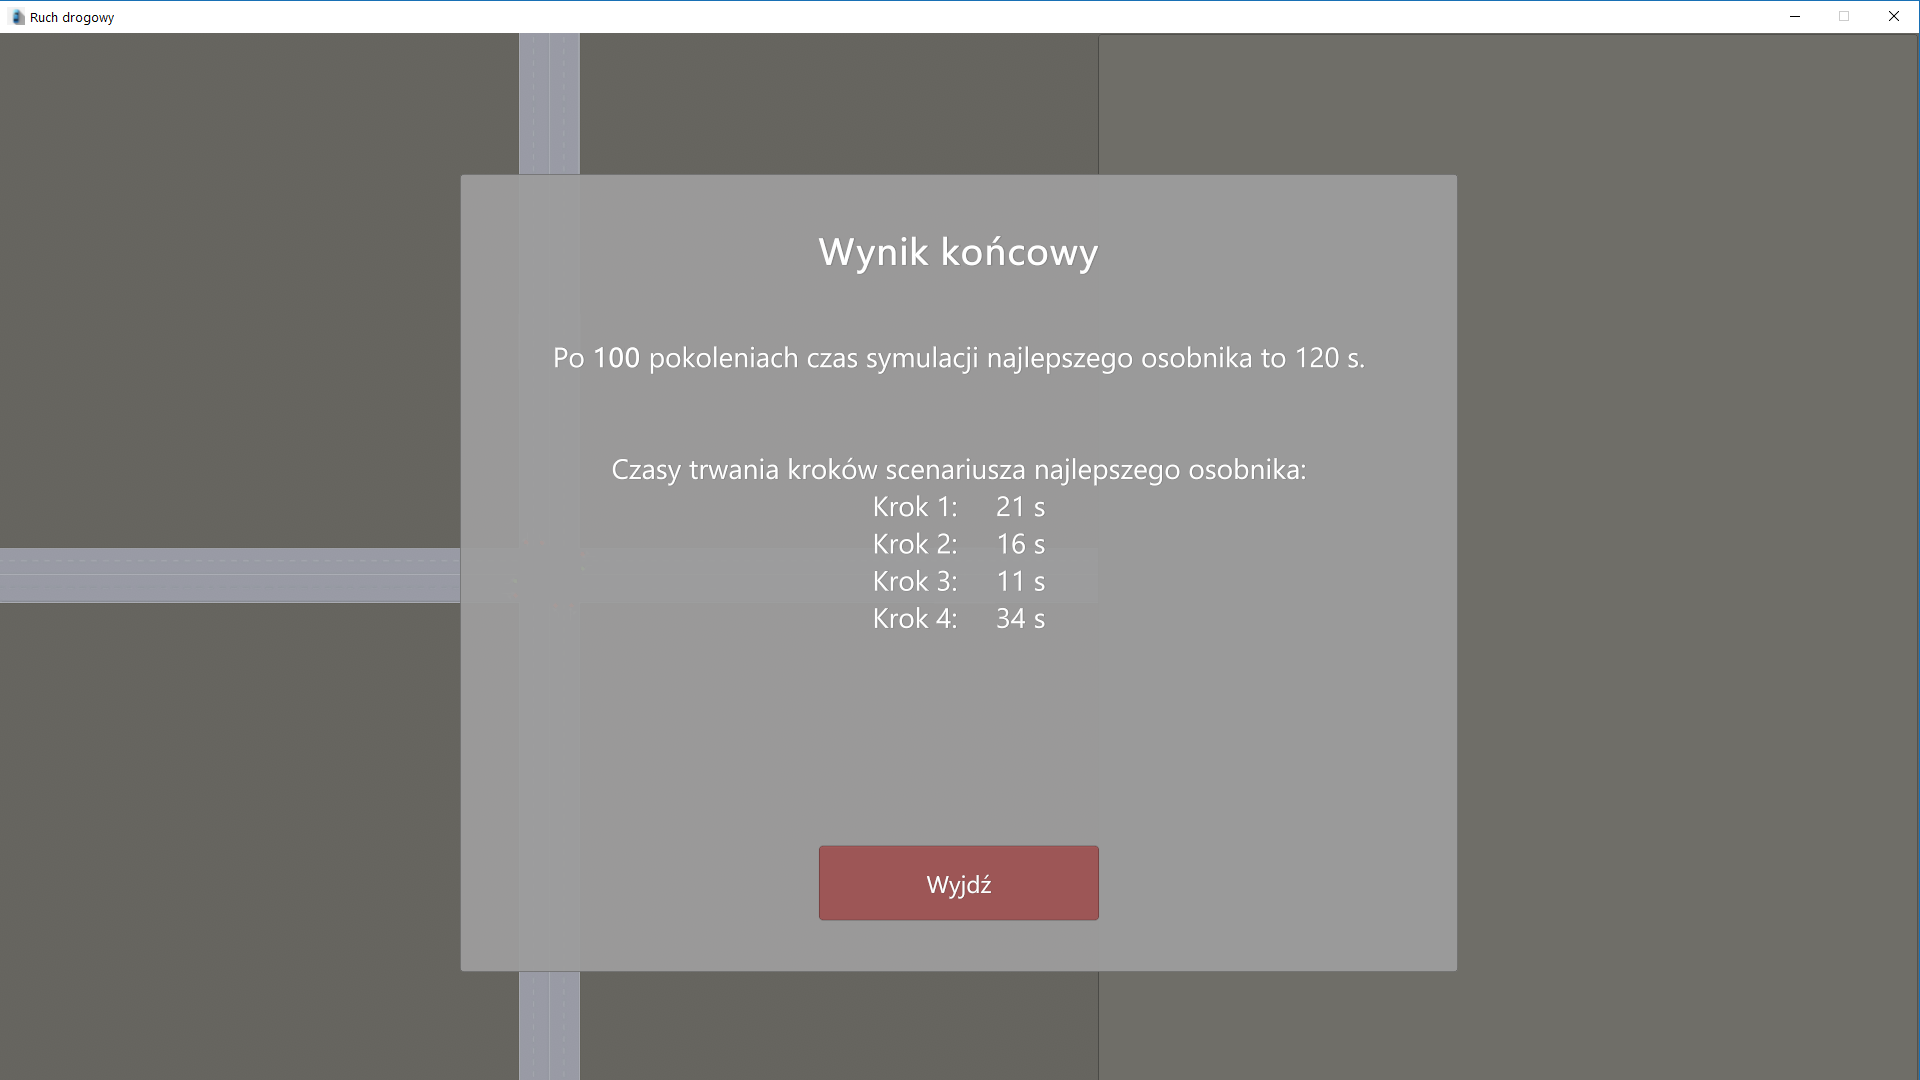
\includegraphics[width=1\linewidth]{ap9}
	\caption[Ekran końcowy]{Ekran końcowy}
	\label{fig:ap9}
\end{figure}

\section*{Ruch pojazdów}
Każdy pojazd porusza się wzdłuż jednej z 12 krzywych sklejanych -- przykładową przedstawiono na rysunku~\ref{fig:ap7} kolorem zielonym. Każda z nich składa się z krzywych Béziera drugiego stopnia.
\section*{Dodatkowe proste narzędzia}Przy okazji powstawania tej aplikacji stworzono proste narzędzie do modyfikacji krzywych sklejanych. Pozwala ono w łatwy sposób przesuwać ich punkty kontrolne w trybie graficznym (co przedstawiono na rysunku~\ref{fig:ap6}) lub wprowadzając ich współrzędne (co ukazuje rysunek~\ref{fig:ap7}).
\paragraph{}Stworzono również narzędzie do szybkiego tworzenia scenariuszy, widoczne na rysunku~\ref{fig:ap8}. Pozwala ono określić liczbę kroków i listę sygnalizatorów, które będą w danym kroku zielone.
\paragraph{}Narzędzia te skróciły czas potrzebny na przygotowanie aplikacji i ułatwiły testowanie różnych rozwiązań.
\begin{figure}
	\centering
	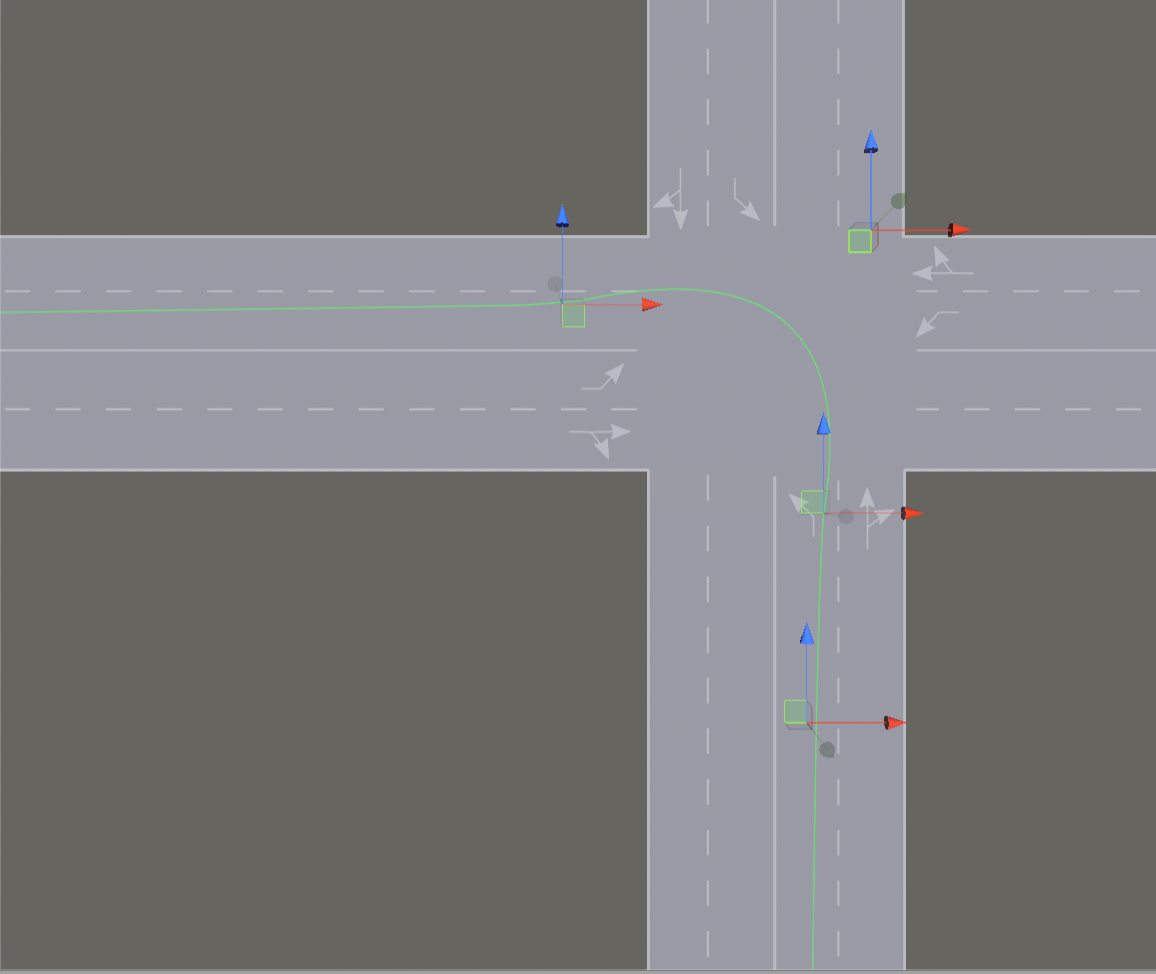
\includegraphics[width=1\linewidth]{ap6}
	\caption[Narzędzie do modyfikacji krzywych sklejanych w trybie graficznym]{Narzędzie do modyfikacji krzywych sklejanych w trybie graficznym}
	\label{fig:ap6}
\end{figure}
\begin{figure}
	\centering
	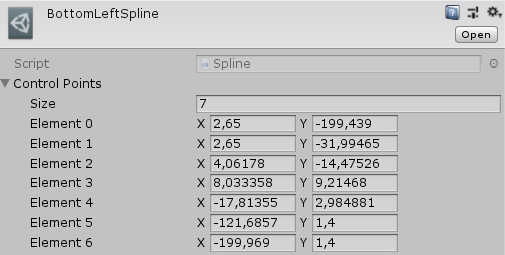
\includegraphics[width=0.8\linewidth]{ap7}
	\caption[Narzędzie do modyfikacji krzywych sklejanych w trybie tekstowym]{Narzędzie do modyfikacji krzywych sklejanych w trybie tekstowym}
	\label{fig:ap7}
\end{figure}
\begin{figure}
	\centering
	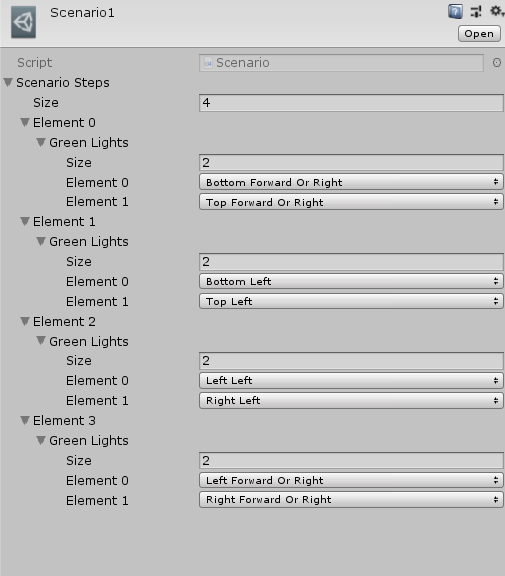
\includegraphics[width=0.8\linewidth]{ap8}
	\caption[Narzędzie do tworzenia scenariuszy]{Narzędzie do tworzenia scenariuszy}
	\label{fig:ap8}
\end{figure}
%Kolejny rozdział wyniki: głównie wykresy
%Podsumowanie
%Streszczenie, abstract i dopisać do wstępu opis rozdziałów




	\chapter*{Wyniki uczenia}
W tym rozdziale przedstawione są przykładowe wyniki uczenia sygnalizacji.\\
Rysunek~\ref{fig:evoA} przedstawia rezultaty z użyciem algorytmu opisanego w rozdziale \textit{Opis teoretyczny algorytmu ewolucyjnego}. W tym przykładzie rozmiar populacji pokolenia wynosił 10 osobników, a pozostałe ustawienia były domyślne. Jeśli porównać najlepszego osobnika  ostatniego i pierwszego pokolenia, to nastąpiła 26-procentowa poprawa czasu.
\pgfplotstableread[col sep = comma]{p10,randOvertapOsc,3tourn10,pr1.csv}\evoA
\begin{figure}[h]
	\centering
	\begin{tikzpicture}
	\begin{axis}
	[
	grid=major,
	width=1\textwidth,
	xlabel=Pokolenie,
	ylabel=Czas najlepszego osobnika {[s]},
	xmin=0,
	xmax=100,
	ymin=0,
	ytick={0,10,...,160}
	]
	\addplot+[mark=none,thick] table {\evoA};
	\end{axis}
	\end{tikzpicture}
	\caption{Wynik uczenia z 10 osobnikami w pokoleniu}
	\label{fig:evoA}
\end{figure}\\
\paragraph{}Rysunek~\ref{fig:evoB} przedstawia wyniki z wykorzystaniem tego samego algorytmu co wyżej, z tą różnicą, że rozmiar turnieju to 2 osobników, a najlepszy osobnik nie przechodził bezwarunkowo do kolejnego pokolenia. Rozmiar populacji pokolenia to ponownie 10 osobników, maksymalny współczynnik mutacji to 0,33, a do pozostałych ustawień użyto domyślnych wartości. Ostatecznie uzyskano tutaj 43-procentowy spadek czasu, jednak to w dużej mierze zasługa wysokiego czasu w pierwszym pokoleniu.
\pgfplotstableread[col sep = comma]{pop10,tapOsc1over3,2tourn10of20.csv}\evoB
\begin{figure}[h]
	\centering
	\begin{tikzpicture}
	\begin{axis}
	[
	grid=major,
	width=1\textwidth,
	xlabel=Pokolenie,
	ylabel=Czas najlepszego osobnika {[s]},
	xmin=0,
	xmax=100,
	ymin=0,
	ytick={0,10,...,200}
	]
	\addplot+[mark=none,thick] table {\evoB};
	\end{axis}
	\end{tikzpicture}
	\caption{Wynik uczenia inną wersją algorytmu}
	\label{fig:evoB}
\end{figure}
\paragraph{}
Z kolei na rysunku~\ref{fig:evoC} przedstawiono wyniki z wykorzystaniem stałego współczynnika mutacji równego 0,1 oraz populacji o rozmiarze 20 osobników. Uzyskano tu jedynie 6-procentowy spadek czasu między pierwszym a ostatnim pokoleniem.
\pgfplotstableread[col sep = comma]{pop20,newermut0.1.csv}\evoC
\begin{figure}[h]
	\centering
	\begin{tikzpicture}
	\begin{axis}
	[
	grid=major,
	width=1\textwidth,
	xlabel=Pokolenie,
	ylabel=Czas najlepszego osobnika {[s]},
	xmin=0,
	xmax=83,
	ymin=0,
	ytick={0,10,...,190}
	]
	\addplot+[mark=none,thick] table {\evoC};
	\end{axis}
	\end{tikzpicture}
	\caption{Wynik uczenia z 20 osobnikami w pokoleniu i stałym współczynnikiem mutacji}
	\label{fig:evoC}
\end{figure}
	\chapter*{Podsumowanie}
Celem pracy było stworzenie aplikacji usprawniającej płynność ruchu drogowego poprzez optymalizację sygnalizacji świetlnej.
\section*{Symulacja ruchu drogowego}
Zaimplementowano symulację ruchu pojazdów reagujących na sygnalizatory i inne pojazdy, odpowiednio hamujących lub przyspieszających w odpowiednich momentach. Ta symulacja stała się podstawą procesu optymalizacji decydując o ocenie każdego rozwiązania. Kod jest na tyle zoptymalizowany, że na współczesnych procesorach symulacja może bezproblemowo być uruchomiona ze 100-krotnym przyspieszeniem. Przy takim ustawieniu 100-pokoleniowy proces uczenia z 10 osobnikami na pokolenie trwa około godziny. Dalszą drogą do zwiększenia wydajności mogłoby być wprowadzenie wielowątkowości -- silnik Unity umożliwia wykorzystanie wszystkich wątków procesora, wymaga to jednak nieco innej struktury kodu i rozważenia przypadków charakterystycznych dla obliczeń równoległych.\\
Głównym wyzwaniem w implementacji symulacji było czasochłonne szukanie błędów w kodzie oraz jego optymalizacja.
\section*{Uczenie sygnalizacji świetlnej}
Zaimplementowano algorytm ewolucyjny, który optymalizuje parametry sygnalizatorów świetlnych. Udostępniono możliwość konfiguracji ustawień algorytmu. Na podstawie rozdziału \textit{Wyniki uczenia sygnalizacji} można stwierdzić, że algorytm jest dość skuteczny w znajdowaniu coraz lepszych rozwiązań. Jego implementacja była największym wyzwaniem w tej pracy, w szczególności dobór odpowiedniej techniki mutacji i krzyżowania osobników. Zastosowany algorytm można rozwinąć, wprowadzając dynamiczną regulację jego parametrów (jak choćby współczynnika mutacji) zależną od tempa postępów uczenia w poprzednich pokoleniach.
\paragraph{} 
Stabilność aplikacji jest na zadowalającym poziomie -- nawet przy wielogodzinnej pracy nie występują błędy.
\paragraph{} 
Postawiony cel pracy udało się osiągnąć, a aplikacja spełnia postawione wymagania funkcjonalne i pozafunkcjonalne. Można ją rozwinąć wprowadzając inne typy skrzyżowań lub dodając możliwość tworzenia własnych scenariuszy przez użytkownika.
	\bibliographystyle{moj}
	\bibliography{bibliografia}
	\listoffigures
	
\end{document}